% !TEX root =  master.tex
\section{Value Proposition Canvas}
Ein Value Proposition Canvas (VPC) stellt eine Ergänzung zum Business Model dar und ist ein Werkzeug, welches das Designen, Testen, Verwalten und Erstellen von Kundenwertversprechen unterstützt. \enquote{Think of the Value Proposition as a contract between the customer and your company where the customer “hires” your company to solve a problem.} (Clayton Christensen) Mit dieser Formulierung bringt Christensen ziemlich genau auf den Punkt, was man unter einem VPC versteht. Es bildet gewissermaßen einen Vertrag zwischen Kunde und Unternehmen, indem es darum geht, ein Problem des Kunden zu lösen. Das VPC hilft nicht nur systematisch das Wertversprechen des Unternehmens herauszuarbeiten, es ist auch Basis für Marketing, Pricing und den späteren Erfolg am Markt. Aus einer Umfrage von Simon \& Kucher aus dem Jahr 2014 geht hervor, dass 72\% aller Produktinnovationen scheitern. Hauptgrund dafür ist die fehlende Wahrnehmung beim Kunden.\autocite[vgl.][]{Simon&Kucher.2014}\\
\begin{figure}[htbp] 
	\centering
	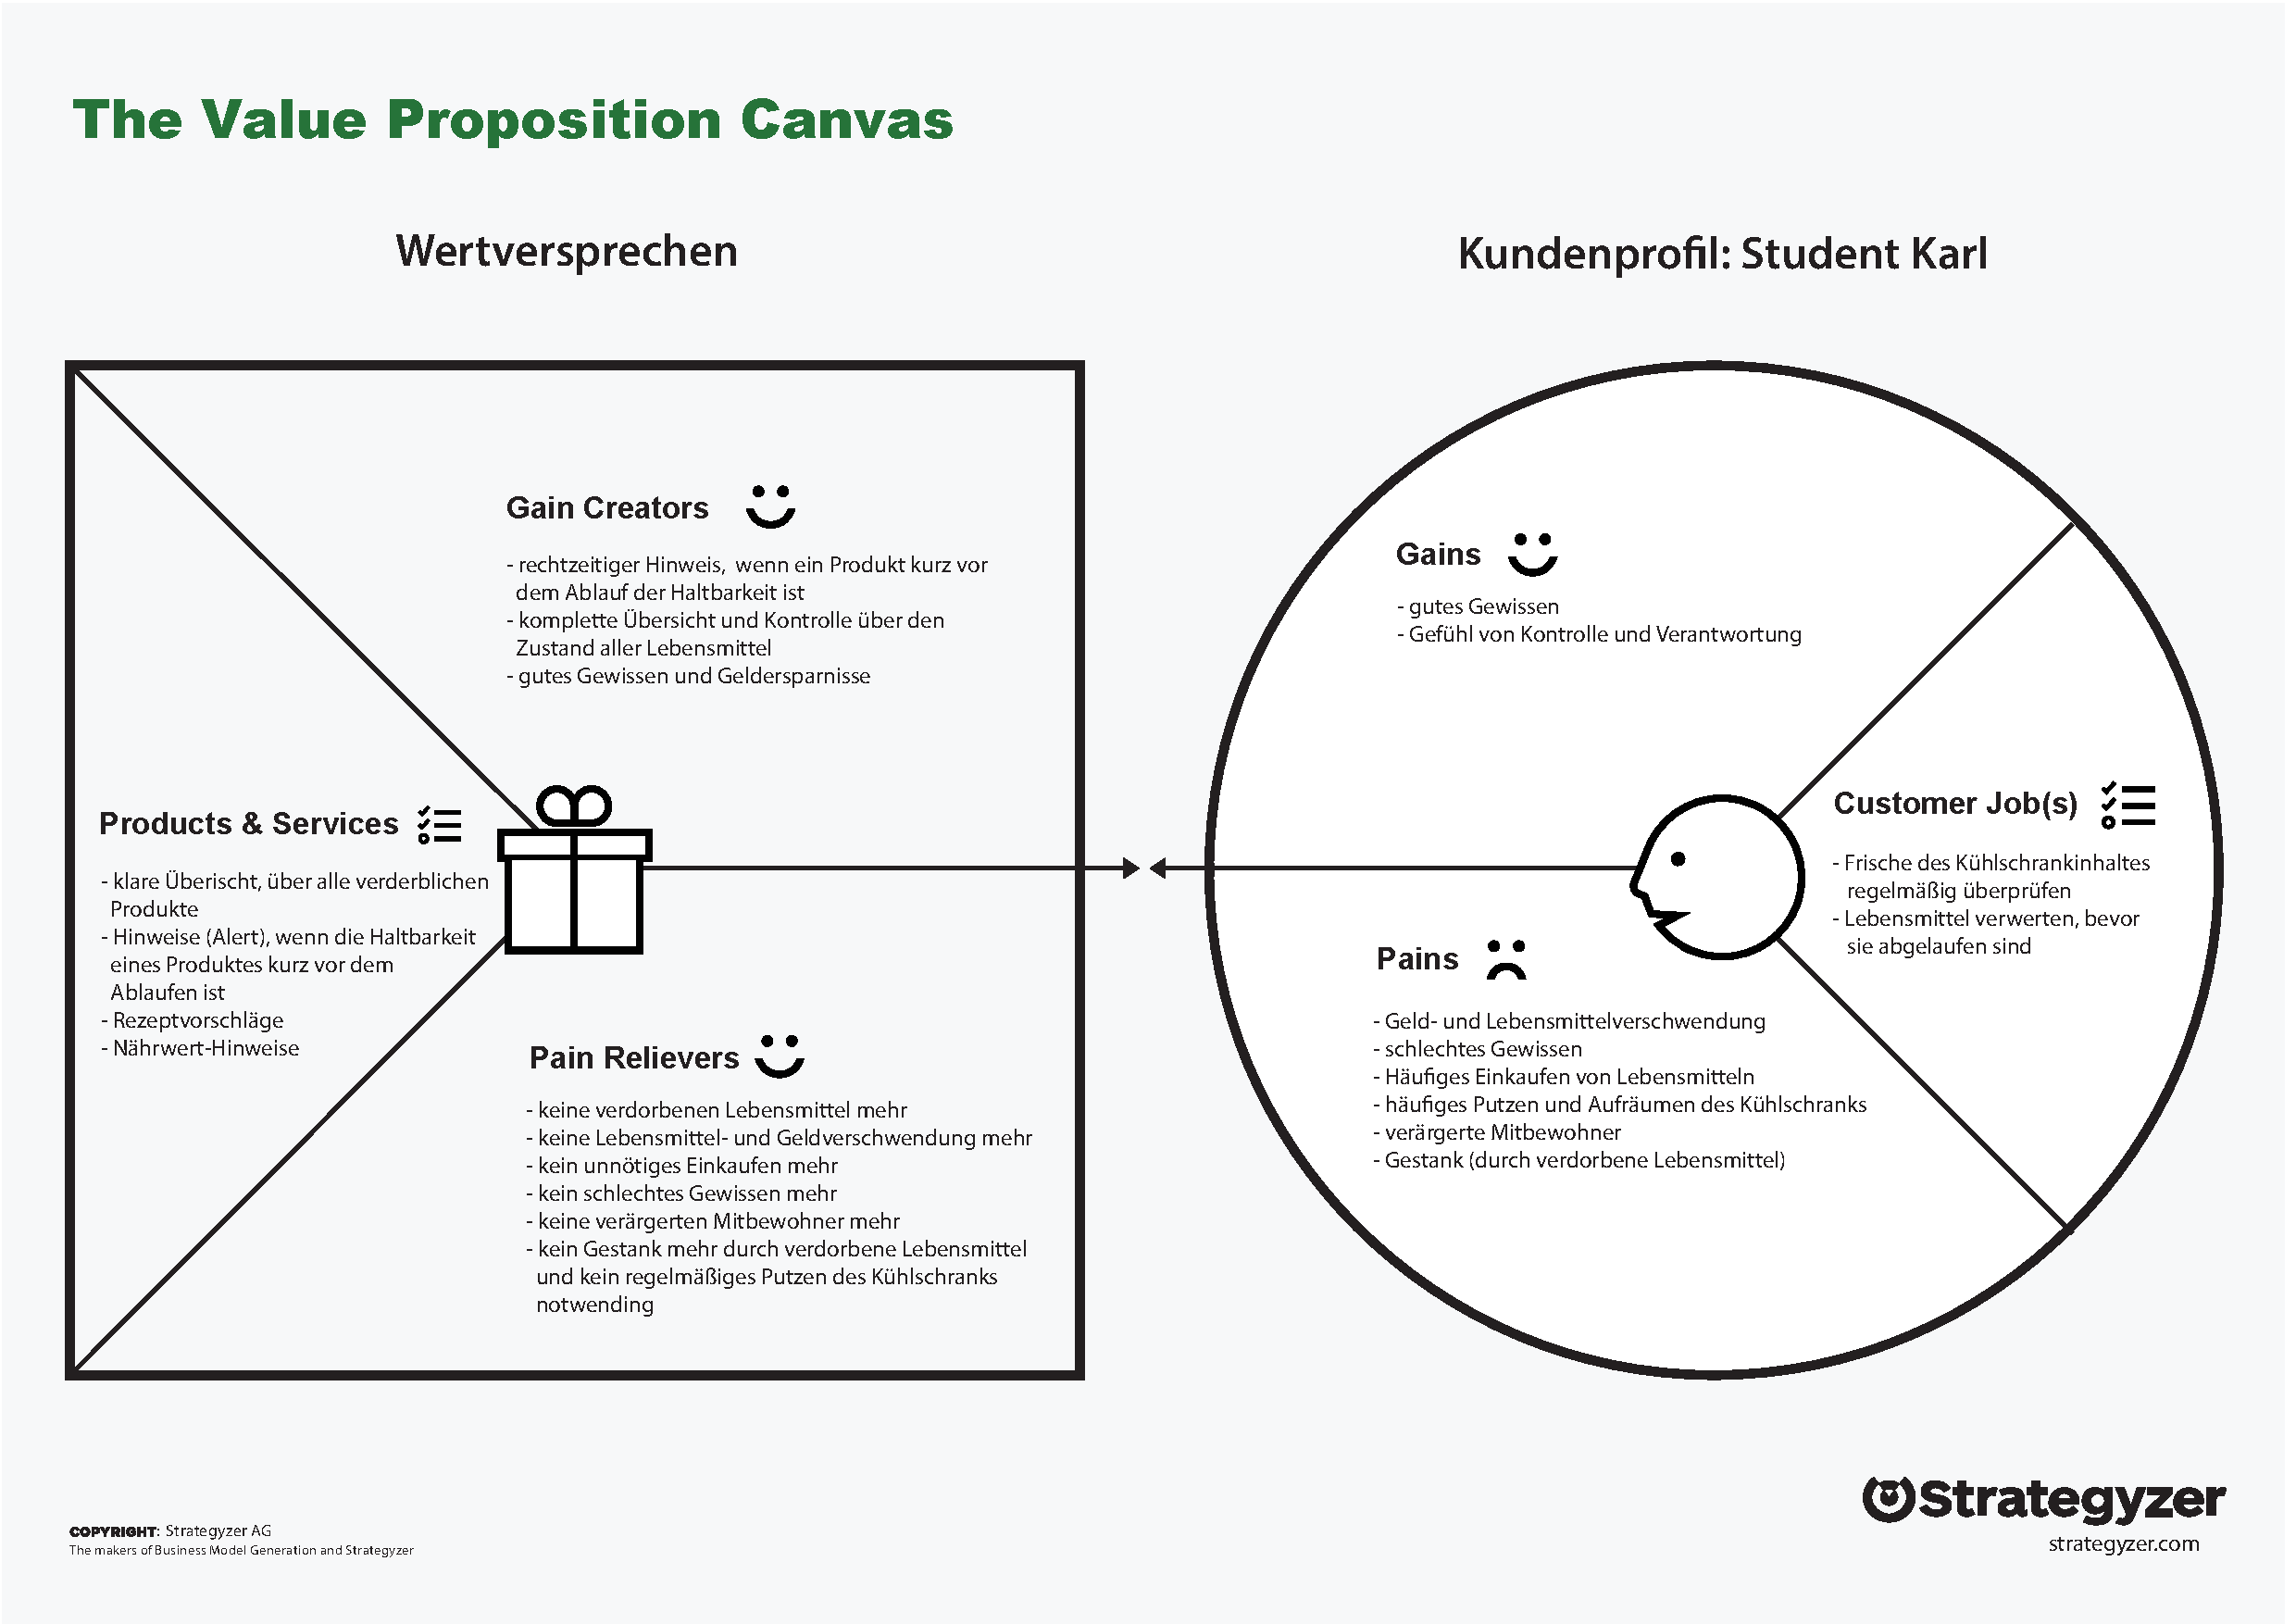
\includegraphics[width=0.8\textwidth]{img/VPC.pdf}
	\caption{Value Proposition Canvas}
	\label{fig:vpc}
\end{figure}

Die Abbildung \ref{fig:vpc} zeigt den Value Proposition Canvas für die Xpire-App. Dabei stehen sich Wertversprechen der App und das Kundenprofiln gegenüber. Die Kundenseite gliedert sich in \enquote{Customer Jobs}, \enquote{Gains} und \enquote{Pains}. Dadurch wird aufgezeigt, welche Aufgaben der Kunde erledigen möchte, warum er diese erledigen möchte und mit welchen Herausforderungen und Schwierigkeiten er dabei konfrontiert wird. Auf der linken Seite des VPC sind die Wertversprechen des Unternehmens zu sehen, unterteilt in \enquote{Gain Creator}, \enquote{Pain Relievers} und \enquote{Products \& Services}.\\
Im vorliegenden Beispiel ist der Kunde ein Student namens Karl, der in einer Wohngemeinschaft wohnt und daher einen Kühlschrank mit seinen Mitbewohnern teilt. Er geht häufig einkaufen, hat meistens Geldprobleme und einen schlechten Überblick über seine Lebensmittel, da er oft gestresst oder unterwegs ist. Zu seinen Jobs (im Haushalt) gehört das regelmäßige Überprüfen des Kühlschranks und das Verwerten der Lebensmittel, bevor sie abgelaufen sind. Das gelingt ihm  meistens leider nicht, weshalb er regelmäßig verdorbene Lebensmittel wegwerfen muss. Dies ist nicht nur eine Form der Lebensmittel- sondern auch der Geldverschwendung und führt bei Karl regelmäßig zu Frust und einem schlechten Gewissen. Zusätzlich ärgern sich seine Mitbewohner über den Gestank im Kühlschrank, wenn mal wieder ein Produkt verschimmelt ist und Karl muss öfter als ihm lieb ist den Kühlschrank putzen. Er wünscht sich, weniger verschwenderisch zu leben mehr Kontrolle über den Stand seiner Lebensmittel zu haben. Er möchte ein gutes Gewissen haben, wenn es um seine Finanzen geht und verantwortungsvoll im Umgang mit Nahrungsmitteln sein.\\
Die mobile Applikation \enquote{Xpire} hilft Karl seine Ziele zu erreichen und sein Verhalten bezüglich der Lebensmittel- und Geldverschwendung zu verbessern. Xpire ermöglicht ihm eine schnelle und einfache Übersicht über den Stand aller seiner Lebensmittel. Zusätzlich erhält er rechtzeitig Hinweise, wenn eines seiner gekauften Produkte kurz vor dem Ablauf der Haltbarkeit steht. Karl hat somit die volle Kontrolle über all seine Lebensmittel und kann nun weniger verschwenderisch leben. Das schont nicht nur seinen Geldbeutel, auch sein Gewissen und seine Mitbewohner freuen sich. Gestank und verschimmeltes Essen im Kühlschrank gehören nun der Vergangenheit an.\\
Mit Xpire können alle gekauften Produkte in der App per Barcode hinterlegt oder manuell eingegeben werden. Die Produktdaten werden anschließend in einer lokalen Datenbank gespeichert. Zu jedem Produkt können zusätzliche Informationen wie Menge, Einkaufsdatum und Verfallsdatum hinterlegt werden. Xpire zeigt dem Benutzer auf übersichtliche Art und Weise all seine hinterlegten Produkte an und benachrichtigt ihn per Push-Notifications, wenn eines seiner Produkte kurz vor dem Ablauf des Haltbarkeitsdatums steht. Zukünftige Features werden Rezeptvorschläge und Hinweise zu Nährwerten enthalten. 


